\begin{figure} [t]
\center
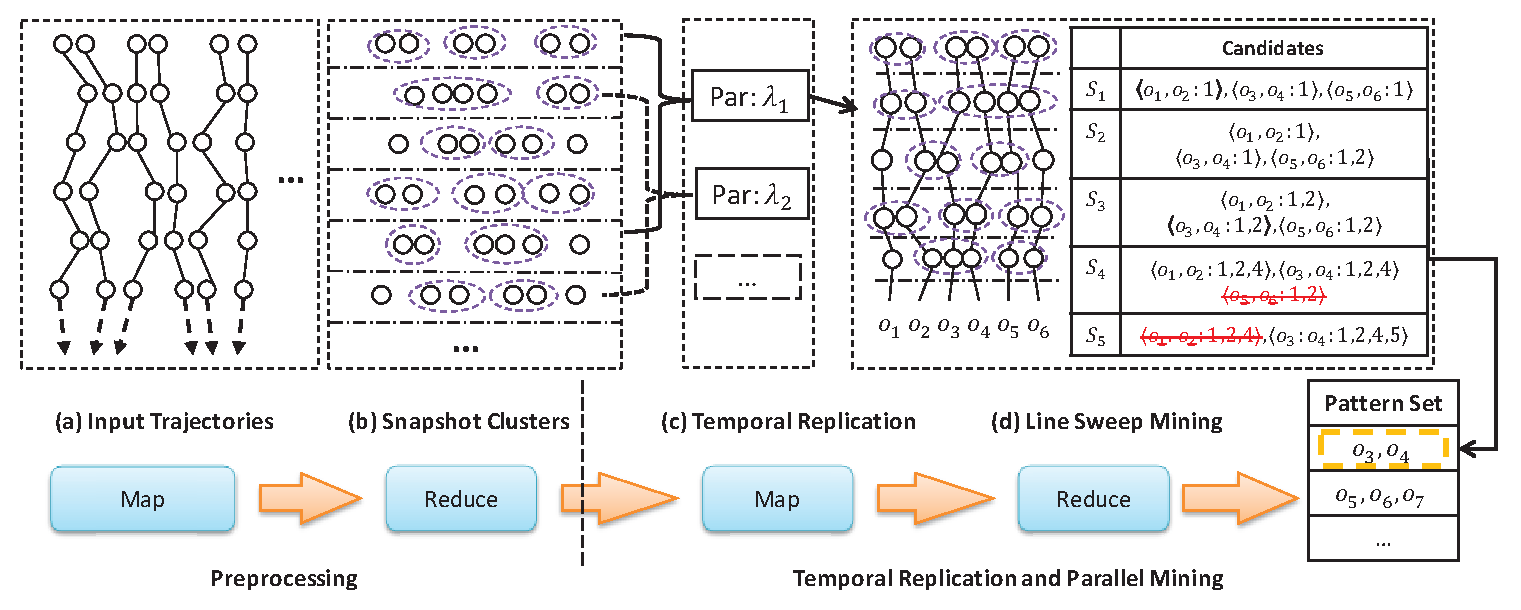
\includegraphics[width=\textwidth]{trm.eps}
    \vspace{-0.5em}
\caption{Workflow of Temporal Replication and Parallel Mining (TRPM). (a) and (b) correspond to the first mapreduce stage which clusters objects in each snapshot.  (c) and (d) correspond to the second mapreduce stage, which uses TRPM to detect GCMPs in parallel.}
\vspace{-0.5em}
\label{fig:trm}
\end{figure}

%\vspace{-3mm}
\section{Baseline: Temporal Replication and Parallel Mining}
\label{sec:trm}
In this section, we propose a baseline solution that resorts to MapReduce as a general, parallel and scalable paradigm for GCMP mining. The framework, named \textit{temporal replication and parallel mining} (TRPM), is illustrated in   Figure~\ref{fig:trm}. There are two stages of mapreduce jobs connected in a pipeline manner. The first stage deals with spatial clustering of objects in each snapshot, which can be seen as a preprocessing step for the subsequent pattern mining phase. In particular, for the first stage, the timestamp is treated as the key in the map phase and objects within the same snapshot are clustered (DBSCAN or disk-based clustering) in the reduce phase. Finally, the reducers output clusters of objects in each snapshot, represented by a list of key-value pairs $\langle t, S_t  \rangle$, where $t$ is the timestamp and $S_t$ is a set of clustered objects at snapshot $t$. 

Our focus in this paper is on the second mapreduce stage of parallel mining, which essentially addresses two key challenges. The first is to ensure effective data partitioning such that the mining on each partition can be conducted independently; and the second is to efficiently mine the valid patterns within each partition. 

It is obvious that we cannot simply split the trajectory database 
into disjoint partitions because a GCMP requires $L$-consecutiveness 
and the corresponding segments may span multiple partitions. 
Our strategy is to use data replication to enable parallel mining. 
Each snapshot will replicate its clusters to $\eta-1$ preceding snapshots.
In other words, the partition for the snapshot $S_t$ contains clusters 
in $S_t$, $S_{t+1}\ldots,S_{t+\eta-1}$. 
Determining a proper $\eta$ is critical in ensuring the
correctness and efficiency of TRPM. If $\eta$ is too small, 
certain cross-partition patterns may be missed. 
If $\eta$ is too large, expensive network communication and 
CPU processing costs would be incurred in the map and reduce phases respectively. Our objective is to find an $\eta$ that is not large but can guarantee correctness.

In our implementation, we set $\eta = (\lceil \frac{K}{L} \rceil - 1)*(G-1)+K+L-1$. Intuitively, with $K$ timestamps, at most $\lceil \frac{K}{L} \rceil - 1$ gaps may be generated as the length of each $L$-consecutive segment is at least $L$. Since the gap size is at most $G-1$, $(\lceil \frac{K}{L} \rceil - 1)*(G-1)$ is the upper bound of timestamps allocated to gaps. The remaining part of the expression, $K+L-1$, is used to capture the upper bound allocated for the $L$-consecutive segments. We formally prove that $\eta$ can guarantee correctness.


\begin{theorem}
\label{THM:RP_ETA}
$\eta = (\lceil \frac{K}{L} \rceil - 1)*(G-1)+K+L-1$ guarantees that no valid pattern is missed.
\end{theorem}

\begin{proof}
Given a valid pattern $P$, we can always find at least one valid subsequence of $P.T$ that is also valid. Let $T'$ denote the valid subsequence of $P.T$ with the minimum length. In the worst case, $T'=P.T$. We define $\range(T)=\max(T) - \min(T) +1$ and prove the theorem by showing that $\range(T') \leq \eta$.
Since $T'$ can be written as a sequence of L-consecutive segments interleaved by gaps: $l_1,g_1,\ldots,l_{n-1}$, $g_{n-1},l_n$ ($n \geq 1$),
where $l_i$ is a segment and $g_i$ is a gap. Then, $\range(T')$
is calculated as $\Sigma_{i=1}^{i=n}|l_i| + \Sigma_{i=1}^{i=n-1} |g_i|$. Since $T'$
is valid, then $\Sigma_{i=1}^{i=n}|l_i| \geq K$. As $T'$ is minimum, if we remove the 
last $l_n$, the resulting sequence should not be valid. Let $K' = \Sigma_{i=1}^{i=n-1}|l_i|$, which
is the size of the first $(n-1)$ segments of $T'$. Then, $K' \leq K-1$.
Note that every $|l_i| \geq L$, thus $n \leq \lceil \frac{K'}{L} \rceil \leq \lceil \frac{K}{L} \rceil $. By
using the fact that every $|g_i| \leq G-1$, we achieve $\Sigma_{i=1}^{i=n-1} |g_i| \leq (n-1)(G-1)
\leq (\lceil \frac{K}{L} \rceil -1)(G-1)$. Next, we consider the difference between $K$ and $K'$, denoted by
$\Delta = K- K'$. To ensure $T'$'s validity, $l_n$ must equal to $\min(L, \Delta)$.
Then, $\Sigma_{i=1}^{i=n}|l_i| = K' + l_n = K - \Delta + \min(L, \Delta) \leq K - 1 + L$. We finish showing $\range(T') \leq \eta$.  Therefore, for any valid sequence $T$, there is at least one valid subsequence with range no greater than $\eta$ and hence this pattern can be detected in a partition with $\eta$ snapshots.
\end{proof}

Based on the above theorem, under TRPM, every consecutive $\eta$ snapshots
form a partition. In other words, each snapshot $S_t$ corresponds to a partition $\lambda_t=\{S_t,...,S_{t+\eta-1}\}$. 
Next, we aim to
%Our next task is to 
design an efficient pattern mining strategy within each partition. Our solution includes a line sweep algorithm to sequentially scan the $\eta$ %replicated 
snapshots in a partition and an effective candidate pattern enumeration mechanism.  

\begin{algorithm}[h]
\caption{Line Sweep Mining}
\label{algo:line-sweep}
\begin{algorithmic}[1]
\Require $\lambda_t = \{S_t, ..., S_{t+\eta-1}\}$
\State{$C \gets \{\}$} \Comment{Candidate set} \label{code:ls-can-set}
\ForAll{clusters $s$ in snapshot $S_t$} 
\label{code:ls-init-start}
\If{$|s| \geq M$}
\State $C\leftarrow C\cup \{\langle s, t \rangle \}$
\EndIf
\EndFor
\label{code:ls-init-end}
\ForAll{$S_j \in \{S_{t+1},\ldots,S_{t+\eta-1}\}$} \label{code:ls-sweep-starts}
	\State $N \gets \{\}$
	\ForAll {$(c,s) \in C \times S_j$} \label{code:ls-join-start}
		\State {$c' \gets \langle c.O \cap s.O, c.T \cup \{j\} \rangle$} \label{code:ls-join}
		\If {$c'.T$ is valid} 
			\State output $c'$
		\ElsIf{$|c'.O| \geq M$}
			\State $N\leftarrow N\cup \{c'\}$ \label{code:ls-m-prun}	
		\EndIf
	\EndFor \label{code:ls-join-ends}
	\ForAll {$c \in C$}
		\If{$j-\max(c.T)\geq G$}\label{code:ls-g-prune-starts}
			\State $C\leftarrow C-\{c\}$ 
			\State output $c$, if $c$ is a valid pattern
		\EndIf  \label{code:ls-g-prune-ends}
		\If{$c$'s first segment is less than $L$}\label{code:ls-l-prune-starts}
			\State $C\leftarrow C-\{c\}$ 
		\EndIf\label{code:ls-l-prune-ends}
	\EndFor
	\State $C\leftarrow C\cup N$
\EndFor\label{code:ls-sweep-ends}
\State output valid patterns in  $C$  \label{code:ls-valid-check}
\end{algorithmic}
\end{algorithm}

Details of the algorithm are presented in Algorithm~\ref{algo:line-sweep}. We keep a candidate set $C$ (Line~\ref{code:ls-can-set}) during the sweeping. It is initialized using the clusters with size no smaller than $M$ in the first snapshot. Then, we sequentially scan each snapshot (Lines~\ref{code:ls-sweep-starts}-\ref{code:ls-sweep-ends}) and generate new candidates by extending the original ones in $C$.
Specifically, we join candidates in $C$ with all the clusters in $S_j$ to form new candidates (Lines~\ref{code:ls-join-start}-\ref{code:ls-join-ends}). 

After sweeping all the snapshots, all the valid patterns are stored in $C$ (Line~\ref{code:ls-valid-check}). 
It is worth noting that $C$ continues to grow during sweeping. We can use three pruning rules to remove  false candidates early from $C$. Since there is a partition $\lambda_t$ for each $S_t$, only patterns that start from timestamp $t$ need to be discovered. Therefore, those patterns that do not appear in the $S_t$ are false candidates. In particular, our
three pruning rules are as follows:
First, when sweeping snapshot $S_j$, new candidates with object set smaller than $M$ are pruned (Line~\ref{code:ls-m-prun}). Second, after joining with all clusters in $S_j$, 
candidates in $C$ with the maximum timestamp no smaller than $j-G$ are pruned (Lines~\ref{code:ls-g-prune-starts}-\ref{code:ls-g-prune-ends}). Third, candidates in $C$ with the size of the first segment smaller than $L$
are pruned (Lines~\ref{code:ls-l-prune-starts}-\ref{code:ls-l-prune-ends}).  
With the three pruning rules, the size of $C$ can be significantly reduced.  

\begin{algorithm}[h]
\caption{Temporal Replication and Parallel Mining}
\label{algo:trm_overview}
\begin{algorithmic}[1]
\Require list of $\langle t, S_t \rangle$ pairs
\State $\eta \gets (\lceil \frac{K}{L} \rceil -1)*(G-1)+K+L-1$
\State {\textit{---Map Phase---}}
\label{code:trm-map-start}
\ForAll{snapshots $S_t$}
	\ForAll{$i \in 1...{\eta-1}$}
		\State emit key-value pair $\langle \max(t-i,0), S_t \rangle$ 
	\EndFor  
\EndFor
\label{code:trm-map-end}
\State {\textit{---Partition and Shuffle Phase---}}
\label{code:trm-par-start}
\ForAll{key-value pairs $\langle t, S \rangle$} 
\State group-by $t$ and emit a key-value pair $\langle t, \lambda_t\rangle$, where $\lambda_t = \{S_t, S_{t+1}, .. S_{t+\eta-1}\} $
\EndFor
\label{code:trm-par-end}
\State {\textit{---Reduce Phase---}}
\label{code:trm-red-start}
\ForAll{key-value pairs $\langle t,\lambda_t \rangle$}
\State call line sweep mining for partition $\lambda_t$
\label{code:trm-red-end}
\EndFor
\end{algorithmic}
\end{algorithm}
\vspace{-0.5em}
The complete picture of TRPM is summarized in Algorithm~\ref{algo:trm_overview}. We illustrate the  workflow of TRPM using Figure~\ref{fig:trm} (c) and (d) with pattern
parameters $M=2, K=3, L = 2, G=2$. By Theorem~\ref{THM:RP_ETA}, $\eta$ is calculated
as $(\lceil \frac{K}{L} \rceil-1) *(G-1)+ K + L - 1 = 5$. Therefore, 
in Figure~\ref{fig:trm} (c), every $5$ consecutive snapshots are combined 
into a partition in the map phase. In Figure~\ref{fig:trm} (d), a line sweep
method is illustrated for partition $\lambda_1$. Let $C_i$ be the candidate set when sweeping snapshot $S_i$.
Initially, $C_1$ contains 
%patterns with 
all object sets in 
%snapshot 
$S_1$.
%As we sweep the snapshots, the patterns in $C_i$ grow.
At snapshot $S_4$, the candidate
$\langle o_5,o_6 \rangle$ is removed because the gap between its latest timestamp (i.e., $2$)
and the next sweeping timestamp (i.e., $5$) is $3$, which violates the $G$-connected constraint.
Next, at snapshot $S_5$, the candidate $\langle o_1,o_2 \rangle$ is removed
because its local consecutive segment $(4)$ has only $1$ element,
which violates the $L$-consecutive constraint.
Finally, $\langle o_3,o_4 \rangle$ is the valid pattern and is returned. Note that in this example, $\eta=5$ is the minimum setting that can guarantee correctness. If $\eta$ is set to be $4$, the pattern $\langle o_3,o_4 \rangle$ would be missed. 




